%\documentclass[11pt,dvipdfm]{article} 
\documentclass[11pt]{article}
%\usepackage[utf8]{inputenc}
\usepackage{deauthor}
\usepackage{times}
\usepackage{graphicx}
\usepackage{multirow}
\usepackage{caption}
%\usepackage[hidelinks]{hyperref}
\usepackage{url}
\usepackage{caption}
\usepackage{subcaption}

\begin{document}

\title{The Anatomy of Blockchain Database Systems}
\author{Dumitrel Loghin \\ National University of Singapore \\ dumitrel@comp.nus.edu.sg}

\maketitle

\begin{abstract}

Blockchains are around for more than ten years and currently, we are witnessing the adoption of blockchain techniques in databases, and vice-versa. For example, typical blockchain data structures, such as cryptographically-linked blocks and Merkle trees, have been integrated into verifiable databases. On the other hand, database techniques, such as sharding and concurrency control, have been integrated into blockchains. In this paper, we are looking at systems that combine both blockchain and database techniques. We classify these systems into (i) permissioned blockchains, (ii) hybrid blockchain database systems, and (iii) ledger databases. We present their anatomy, including features, techniques, and design choices, by analyzing a few representative systems. In the end, we highlight their limitations and discuss future research directions.

\end{abstract}
 
\section{Introduction}

In the last few years, the line between blockchain systems and distributed databases has been blurred to a certain degree~\cite{rpc_sigmod21, sharma_sigmod19}. We have seen the adoption of blockchain techniques in databases. For example, typical blockchain data structures, such as cryptographically-linked blocks~\cite{fabric} and Merkle trees~\cite{merkle_tree}, have been integrated into verifiable ledger databases~\cite{qldb, sqlledger2021, ledgerdb, spitz} and hybrid blockchain database systems~\cite{loghin_vldb2022}. We have also seen database techniques used in blockchains. For example, sharding is used to scale blockchains~\cite{anh_sigmod19}, while optimistic concurrency control (OCC) is used to decrease the number of aborted transactions~\cite{sharma_sigmod19, rpc_sigmod20}.

By zooming into the design and implementation of systems that combine blockchain and database techniques, we propose classifying them into three categories. Going from systems that have stronger blockchain features to systems that are closer to databases, these three categories are (i) \textit{permissioned blockchains}, (ii) \textit{hybrid blockchain database systems}, and (iii) \textit{ledger databases}. From a high-level view, all these systems consist of distributed server nodes that communicate via a broadcasting service based on some consensus protocol. Each server node has a ledger (blockchain data structure) and a local database. Both the server nodes and the users (or clients) that interact with these nodes need to be authenticated. The broadcasting service is implemented either with a Crash Fault Tolerant (CFT) consensus protocol, that is closer to distributed databases, or a Byzantine Fault Tolerant (BFT) consensus that resembles typical blockchains.

In this paper, we analyze a few representative systems and present their anatomy in terms of design, techniques, features, and limitations. We shall present more details on our classification in Section~\ref{sec:class}, and analyze a few systems in Section~\ref{sec:anatomy}. We present challenges, limitations, and future research directions in Section~\ref{sec:challenges}, and conclude in Section~\ref{sec:concl}.


\section{Classification}
\label{sec:class}

When analyzing the systems that combine both database and blockchain techniques, we can distinguish three main categories. First, we have \textit{permissioned blockchains} (also known as private, enterprise, or consortium) that have more blockchain features than databases. Second, we have \textit{hybrid blockchain database systems} which can be further classified into out-of-blockchain databases and out-of-database blockchains~\cite{rpc_sigmod21}. Third, we have (centralized) \textit{ledger databases}. Table~\ref{tab:class} presents the features of such systems and a few examples of the state-of-the-art for each category.


\begin{table}[tp]
    \centering
    \caption{Categories, Features, and Examples.}
    \label{tab:class}
    \resizebox{0.99\textwidth}{!}{
    \begin{tabular}{|l|c|c|c|}
         \hline
         & \textbf{Permissioned Blockchains}
         & \textbf{Hybrid Blockchain Database Systems}
         & \textbf{Ledger Databases} \\
         \hline
         \hline
         Administration & Decentralized & Decentralized & Centralized \\
         Broadcasting & CFT or BFT & Typically CFT & CFT \\
         Local Database & Tightly-coupled & Loosely-coupled & Tightly-coupled \\
         Ledger & Replicated & Replicated & Centralized \\
         \hline
         \hline
         \multirow{6}{*}{Examples} & & Veritas~\cite{veritas_cidr19} & Amazon QLDB~\cite{qldb}  \\
         & Fabric~\cite{fabric} & BigchainDB~\cite{bigchaindb_wp} & Alibaba LedgerDB~\cite{ledgerdb} \\
         & Quorum~\cite{quorum_code} & BlockchainDB~\cite{blockchaindb} & Microsoft SQL Ledger~\cite{sqlledger2021} \\
         & Corda~\cite{corda} & Blockchain Relational Database~\cite{brd} & Spitz~\cite{spitz} \\
         & Diem~\cite{diem_page} & ChainifyDB~\cite{chainifydb} & Immudb~\cite{immudb} \\
         & & FalconDB~\cite{falcondb} & IntegriDB~\cite{integridb} \\
         \hline
    \end{tabular}
    }
\end{table}

\textbf{Permissioned blockchains}, as opposed to typical permissionless or private blockchains such as Bitcoin~\cite{Bitcoin_2008} and Ethereum~\cite{Ethereum_2013}, employ authentication for the parties using the blockchain (i.e., clients and peers). They are named permissioned or private blockchains because only authenticated parties can use them. These blockchains are typically used in enterprise setups and they are operated by a consortium of organizations, hence, they are called enterprise or consortium blockchains. In such setups, an organization hosts one or more blockchain peers (or nodes). Since more than one organization is in charge of administrating and operating the blockchain, a permissioned blockchain is a decentralized system where the ledger is replicated on all the nodes (or peers). Initially, some of these permissioned blockchains considered using Byzantine Fault Tolerant (BFT) consensus protocols to replicate the ledger. For example, Hyperledger Fabric v0.6~\cite{anh_tkde18, anh_sigmod17} used PBFT~\cite{pbft} and Quorum provides support for IBFT~\cite{ibft}. However, these BFT protocols degrade the performance of a blockchain concerning throughput and latency~\cite{anh_sigmod17, loghin_green2019}. That is why most of the current permissioned blockchains use Crash Fault Tolerant (CFT) consensus mechanisms, such as Raft~\cite{raft} and Apache Kafka~\cite{kafka_site}.

\textbf{Hybrid Blockchain Database Systems} are very similar to permissioned blockchains but they have different motivations, use cases, and database integration. These systems are motivated by the need of organizations to share a database or parts of a database. In general, this database already exists and it is loosely-coupled to the hybrid blockchain database system. For example, in a supply chain scenario, there should be a shared database with shipping options and costs. Shipping companies update this database, while the other parties just read the data. In such a case, we need a ledger to keep track of the updates in a transparent and tamper-evident way. An authentication mechanism is needed to access the ledger and the broadcasting service. Given this, most of the proposed hybrid blockchain database systems consider only CFT broadcasting services. As expected, if a BFT consensus is used instead, the performance of the system significantly degrades~\cite{loghin_vldb2022}.

\textbf{Ledger Databases} are at the other end of the centralized-decentralized administration spectrum since they are hosted and operated by a single organization. In such a centralized model, the users need to trust that organization. To increase the trust, ledger databases use tamper-evident data structures and publish the hashes of the append-only ledger or provide proofs for current states in the database. Such systems may be distributed to increase fault tolerance and improve performance. However, they are not distributed to increase the trust as is the case for the other two categories. Moreover, the database and the ledger are tightly-coupled to the server nodes. While such systems require higher trust from the users, they provide higher performance and zero administration efforts compared to the other two categories.


\section{Anatomy}
\label{sec:anatomy}

In this section, we start with the similarities among the three proposed categories, after which we present the particularities of each category together with the details of a few representative systems.

\begin{figure}[tp]
	\centering    
	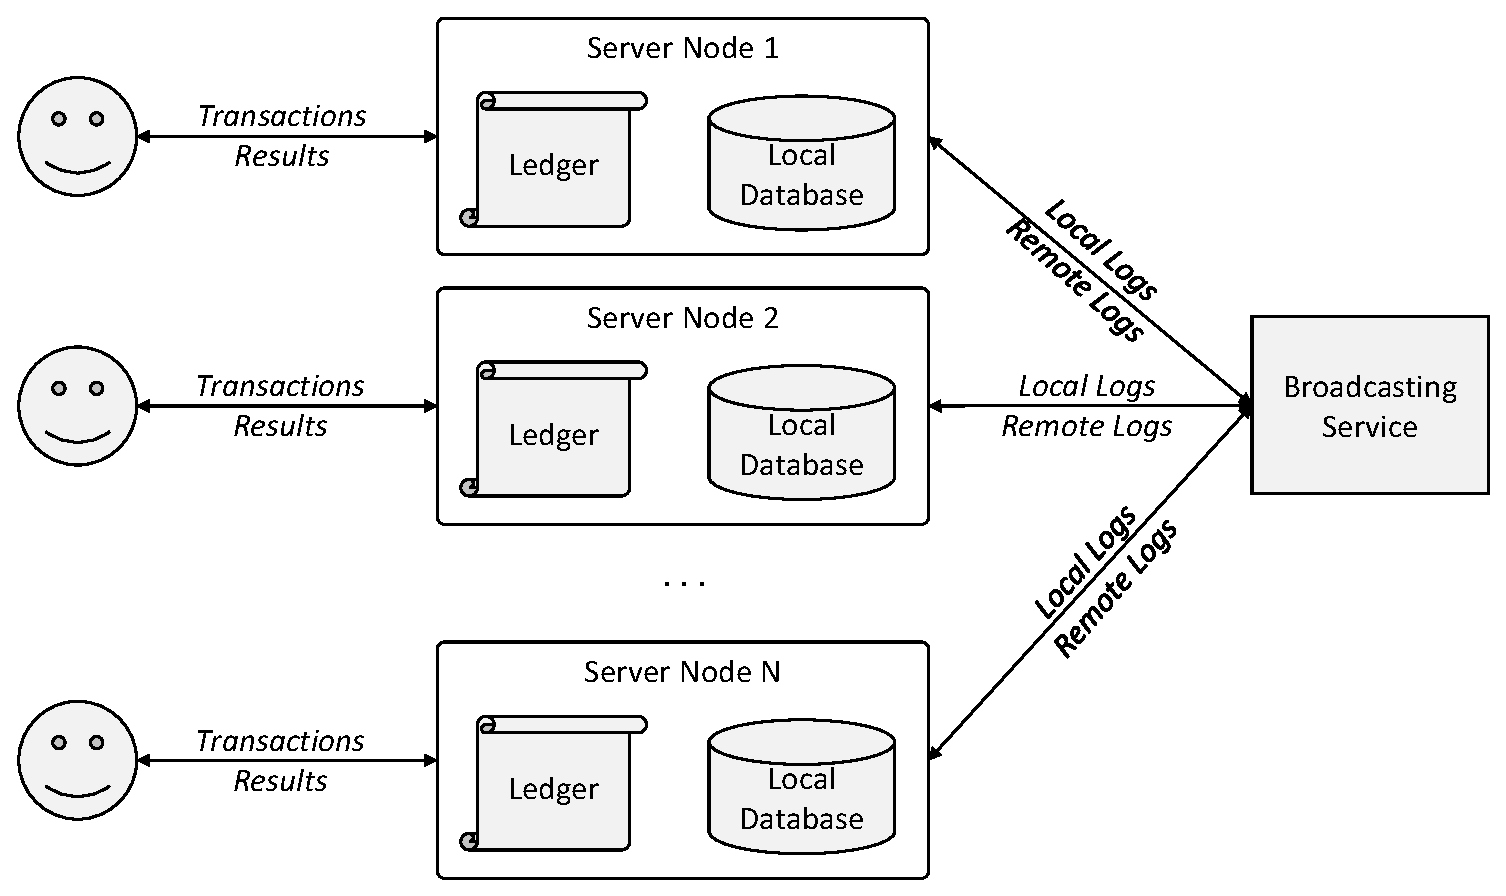
\includegraphics[width=0.85\textwidth]{figs/veritas-digram.eps}
	\caption{A Generic Hybrid Blockchain Database System}
    \label{fig:hbdb}    
\end{figure}

\subsection{Overview}

Typically, systems that combine blockchain and database features have an architecture similar to the one depicted in Figure~\ref{fig:hbdb}. The system consists of some distributed server nodes (or peers), where each node handles user requests and coordinates with the other nodes via a broadcasting service. The users (or clients) need to be authenticated before sending requests to the nodes. A server node sends local updates (or logs) to and receives remote updates (or logs) from the broadcasting service. This broadcasting service can also be distributed across a few nodes, not necessarily the same as the server nodes. Moreover, the broadcasting service is implemented with a CFT or BFT consensus protocol. For example, the latest version of Fabric uses Raft~\cite{raft}, which is CFT, while Quorum supports, among others, IBFT~\cite{ibft}.

Each server node connects to a local database and keeps a copy of the distributed ledger. Note that the local database and the ledger are different. The former keeps the latest version of the data (e.g., states, accounts, assets), while the latter keeps the entire update history using tamper-evident data structures. For example, Fabric uses LevelDB or CouchDB as its local database, which is also called World State. On the other hand, the ledger in Fabric is a linked list of blocks where the header of a block is linked to the header of the previous block using a cryptographic hash. Other systems use data structures based on Merkle trees~\cite{merkle_tree} to represent the ledger.

% https://hyperledger-fabric.readthedocs.io/en/latest/ledger/ledger.html
\begin{figure}[tp]
	\centering
	\begin{subfigure}{0.48\textwidth}
	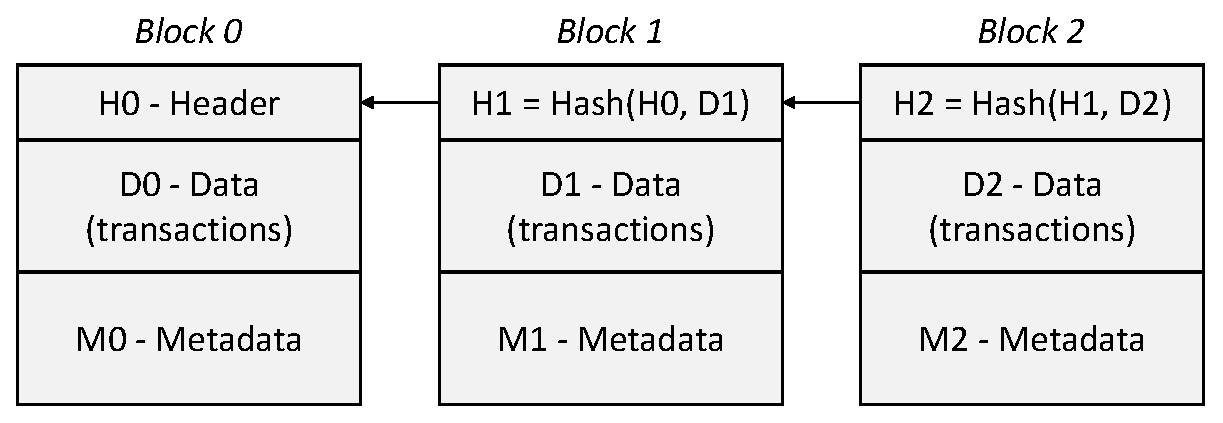
\includegraphics[width=\textwidth]{figs/blocks_diagrams.eps}
	\caption{Hashed Blocks}
	\label{fig:blocks}    
	\end{subfigure}
	\quad
	\begin{subfigure}{0.48\textwidth}
	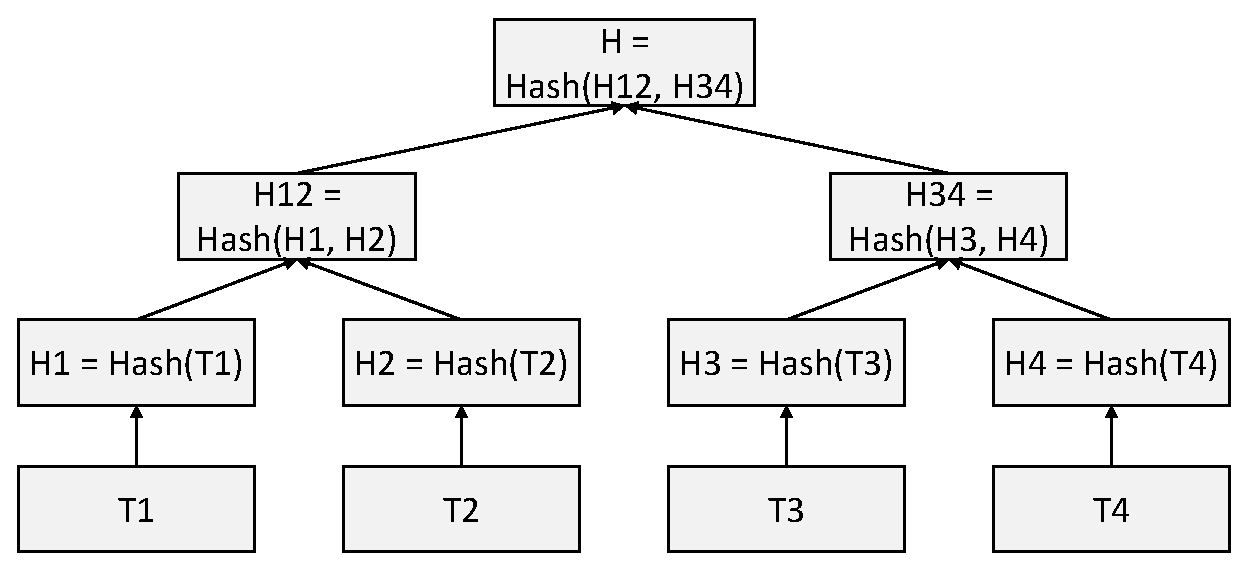
\includegraphics[width=\textwidth]{figs/merkle_diagram.eps}
	\caption{Merkle Tree}
	\label{fig:merkle}  
	\end{subfigure}
	\caption{Ledger Data Structures}
    \label{fig:ledgers}    
\end{figure}

We briefly compare these two ledger data structure, as illustrated in
Figure~\ref{fig:ledgers}. The hashed blocks data structure, as shown in
Figure~\ref{fig:blocks}, is a linked list of blocks where a block points to its
predecessor using a cryptographic pointer, except for the first block which is
typically called the \textit{genesis} block. Each block consists of data,
metadata, and header sections. The data section contains all the transactions
that are part of the block. The header is a digest of the block computed using a
hashing function. Most of the blockchains use SHA3 or Keccak hashing algorithms.
The header of all the blocks except the first one is computed as the hash of the
concatenation between the hash of the previous block and the hash of the current
block's data section.

A generic Merkle tree, as shown in Figure~\ref{fig:merkle}, is a tree where the
leaves are data representing transactions and the internal nodes are hashes.
Each parent node contains the hash of the concatenation of all the hashes of its
children. Hence, the root node contains the hash that represents all the
underlying transactions. We note that Merkle trees can be combined with hashed
blocks: the data section of a block can be organized as a Merkle tree. For
example, Quorum uses this approach to store transactions in its ledger. In
contrast, Fabric does not use a Merkle tree: it just hashes the transaction data
as a chunk~\cite{fabric_ledger}. We direct the reader to~\cite{mpt} for an
analysis of advanced Merkle tree data structures.

\subsection{Permissioned Blockchains}

Hyperledger \textbf{Fabric}~\cite{fabric} is a permissioned blockchain developed by Linux Foundation with a significant contribution from IBM. In Fabric, there are three types of nodes, namely, clients, peers, and orderers. A client sends a transaction request to a set of peers governed by an endorsement policy. 
For example, the \textit{AND} policy includes all the peers in the network. That is, a client has to send the transaction to and receive endorsements from all the peers. 
A peer executes the transaction request in simulation mode and creates read and write sets to mark which world states are touched by the transaction. Since this is in simulation mode, the peer does not persist the changes to its local database. Then, the client sends the responses from the peers together with its transaction to the orderers. These orderers pack the transaction in a block and broadcasts the block to all the peers in the network. Currently, Fabric adopts the Raft CFT consensus among orderers. In the last phase, all the peers validate the block and persist the changes of valid transactions to the local database. Note that the peers do not need to re-execute the transaction: they only persist the write set. In the validation phase, the read set is also verified to check if any state has been modified since the transaction was simulated. In such a case, the transaction is aborted. In summary, Fabric implements an execute-order-validate (EOV or XOV) transaction lifecycle, as opposed to many other blockchains that adopt an order-execute (OX) lifecycle. Fabric supports both LevelDB (default) and CouchDB for the world states database. The ledger is stored on the filesystem as a linked list of blocks, where the block headers are linked together via hashing.

Fabric has been extensively analyzed and optimized by the database research community. Many works benchmark and analyze the performance bottlenecks of Fabric~\cite{chacko_sigmod21, anh_tkde18, anh_sigmod17, loghin_green2019, loghin_green2022, thakkar_2018}. In our recent work~\cite{loghin_green2022}, we show that a Fabric network with up to 10 peers can reach around 1,000 transactions-per-second (TPS). Other works improve the rate of aborted transactions by relaxing the concurrency model (e.g., using optimistic concurrency control) and by re-ordering the transactions~\cite{rpc_sigmod20, sharma_sigmod19}.


\textbf{Quorum}~\cite{quorum_code} is a permissioned blockchain that draws its source code from Ethereum (implemented in the Go programming language). Naturally, Quorum supports Solidity smart contracts, but it replaces the energy-inefficient Proof-of-Work consensus with a few alternatives, out of which Raft is the default. Besides Raft, Quorum also supports IBFT (Istanbul BFT), QBFT (Quorum BFT), and Clique Proof-of-Authority (POA). IBFT is inspired by PBFT~\cite{pbft}, while QBFT is an optimized version of IBFT which is also interoperable with Hyperledger Besu, an Ethereum client developed by the Hyperledger Foundation. As opposed to Fabric, Quorum has only peers and clients and adopts the traditional order-execute (OX) transaction lifecycle.
That is, a transaction is first grouped into a block and then executed by each peer in the network. Similar to Fabric, Quorum uses LevelDB as its local database, but it adopts Merkle Patricia Trie for the ledger. In our recent work~\cite{loghin_green2022}, we show that Quorum with Raft exhibits a throughput of 250 TPS, which is relatively low for a permissioned blockchain.


\textbf{Corda}~\cite{corda} is advertised as a distributed ledger technology (DLT) for enterprises. For that reason, it is built on Java and Kotlin so it can be better integrated with existing Java enterprise systems. Besides nodes, a Corda network has notaries which are responsible for validating transactions in terms of uniqueness and validity. In essence, uniqueness prevents double-spending, while validity means that the transaction passes the input-output tests and it has all the required signatures. Notaries use a consensus protocol which is Raft-based in the default version of Corda. This default version uses H2, a relational database management system written in Java, for the local database. The ledger uses a custom version of Merkle trees to hide transaction details from the entities that are not involved in the transaction. A recent publication shows that the performance of Corda is very low, at 15 TPS~\cite{perf_iot20}. Even when a single notary is used to minimize the impact of consensus, the performance is low due to a synchronous (blocking) transaction processing mechanism~\cite{perf_iot20}. 


\textbf{Diem}~\cite{diem_page} is a permissioned blockchain that was developed by a consortium of companies led by Facebook. It was previously known as the \textit{Libra} blockchain~\cite{diem_page}. The entire project has been discontinued in 2022. However, Diem implements some powerful features which are worth mentioning. For example, it uses LibraBFT~\cite{Baudet2019StateMR}, a BFT consensus based on Hotstuff~\cite{hotstuff} which further improves PBFT~\cite{pbft}. For the ledger, Diem uses Jellyfish Merkle tree~\cite{jmt_diem} which is a sparse Merkle tree inspired by the Merkle Patricia Trie used in Ethereum. RocksDB~\cite{rocksdb_paper}, a fast key-value store derived from LevelDB and developed by Facebook, is used as the underlying database. A recent study shows that Diem achieves around 600 TPS on 4 nodes~\cite{perf_diem}, which is a decent performance for a BFT-based blockchain.


\subsection{Hybrid Blockchain Database Systems}

\textbf{Veritas}~\cite{veritas_cidr19} is an out-of-blockchain database that consists of a shared database (or table) and a blockchain ledger for keeping auditable and verifiable updates done on the shared database. Each node is operated by an organization. A node uploads its local update logs and downloads remote update logs to and from a broadcasting service. Veritas employs a concurrency control mechanism based on timestamps. The timestamp of a transaction represents the sequence number of that transaction in the log. A transaction is first verified locally by the node receiving it. If it passes the verification (e.g., multi-version concurrency control -- MVCC), it is included in the logs and sent to the broadcasting service. Once the other nodes agree to the updates, they send acknowledgments, and once every node receives the acknowledgments, it persists the updates to the local database and appends them to the ledger. Note that this mechanism incurs $O(N^2)$ communication complexity~\cite{loghin_vldb2022}.

The original design of Veritas uses Redis~\cite{redis_book}, an in-memory NoSQL database, and Apache Kafka~\cite{kafka_site}, a CFT broadcasting service. The re-implementation of Veritas in~\cite{loghin_vldb2022} achieves around 30,000 TPS, making it the fastest system among all those analyzed in this paper.


\textbf{BlockchainDB}~\cite{blockchaindb} is an out-of-blockchain database with prominent blockchain features: it is a shared database built over a blockchain. It is the only hybrid blockchain database that uses sharding to partition the shared database. Firstly, the blockchain represents the storage layer of a BlockchainDB node. By default, BlockchainDB uses Ethereum, but other blockchains can be used as well via a plugin interface. With Ethereum, the ledger structure is based on Merkle Patricia Trie. Secondly, a node has a database layer with a simple key-value interface. Thirdly, there is a shard manager that helps the database layer to identify the shard where a specific key is stored. Due to the use of such a slow blockchain, like Ethereum with Proof-of-Work (PoW) or Proof-of-Authority (PoA), BlockchainDB exhibits a throughput of around 50 TPS~\cite{loghin_vldb2022}.


\textbf{FalconDB}~\cite{falcondb} is another out-of-blockchain database that starts from a blockchain and provides a shared database to the clients. Different from other systems, FalconDB provides a relational database interface to the clients. In FalconDB, both the clients and the peers need to keep a digest of the data. The difference is that clients only keep the blockchain headers to save storage space. However, these headers are sufficient for checking the correctness of the data queried from the peers. FalconDB uses IntegriDB~\cite{integridb}, a verifiable SQL database, to store the ledger, Tendermint for consensus, and MySQL as the local database. The throughput of the system with a YCSB write-heavy workload (50\% reads and 50\% writes) is around 3,000 TPS~\cite{falcondb}. Note that a similar YCSB workload is used to evaluate Veritas, BigchainDB, and BlockchainDB~\cite{loghin_vldb2022}.


Blockchain Relational Database (\textbf{BRD})~\cite{brd} has a similar design to Veritas, but it starts from a PostgreSQL~\cite{postgresql_site} relational database. In this sense, BRD is an out-of-database blockchain. Also, different from Veritas, the broadcasting service orders blocks of transactions (updates) and does not serialize the transactions in a block. To speedup transaction execution, BRD implements concurrent execution with Serializable Snapshot Isolation (SSI). Note that BRD uses PostgreSQL~\cite{postgresql_site} as its local database, which supports Serializable Snapshot Isolation. BRD also uses Apache Kafka as the broadcasting service. Different from Veritas, BRD keeps the ledger in the same relational database, namely PostgreSQL. According to the BRD paper~\cite{brd}, the system achieves a throughput of 2,500 TPS with a key-value workload.


\textbf{BigchainDB}~\cite{bigchaindb_wp} is another out-of-database blockchain. It starts from MongoDB~\cite{mongodb}, a NoSQL database, used as the local database. By using MongoDB, the main data abstraction in BigchainDB is an asset, represented in JSON format. Otherwise, the transaction lifecycle is similar to the one in Veritas. A transaction is verified locally by a node, then a request is sent to the broadcasting service. BigchainDB uses a BFT consensus middleware as the broadcasting service, namely  Tendermint~\cite{tendermint_thesis}. Once the majority of the nodes agree on the transaction, it is committed in the local database. BigchainDB relies on Tendermint to keep the ledger in the form of a Merkle tree. Our evaluation of the open-source BigchainDB code shows a maximum performance of around 200 TPS with the YCSB workloads.


\textbf{ChainifyDB}~\cite{chainifydb} is an out-of-database blockchain that starts from a relational database which can be either PostgreSQL or MySQL. Apache Kafka is used for broadcasting the transactions which are SQL statements. The ledger uses a custom representation based on LedgerBlocks. A LedgerBlock contains all the transactions that are part of a block, where a transaction is in its SQL form. Next, the LedgerBlock contains a list of bits representing the successful transactions, a SHA256 hash digest over the data changed by the transactions, and a hash value of the previous LedgerBlock that was added to the ledger. This representation is similar to the one used by Fabric. ChainifyDB achieves a throughput of around 1,000 TPS on three nodes using the SmallBank workload when all three nodes need to reach consensus. When only two out of three nodes need to reach consensus, the throughput increases to around 5,000 TPS~\cite{chainifydb}.


\subsection{Ledger Databases}

Amazon Quantum Ledger Database \textbf{QLDB}~\cite{qldb} is a verifiable database developed by Amazon and provided as a cloud service. QLDB follows the structure depicted in Figure~\ref{fig:hbdb} by integrating a relational database and a ledger in its server node. The database keeps the current states and the history of those states, while the ledger is an append-only journal that keeps track of all the changes done to the database in an immutable way. While it is not clear what is the underlying database, the ledger in QLDB is implemented based on Merkle trees. Our preliminary evaluation of QLDB shows a throughput of 10,000 TPS, which is relatively low for a centralized system. However, we note that an update in QLDB changes both the database and the ledger, and these two changes are done sequentially. 


\textbf{LedgerDB}~\cite{ledgerdb} is a verifiable database developed by Alibaba and provided as a cloud service. LedgerDB updates the ledger, which is based on a Merkle tree, asynchronously. Specifically, the transactions are batched and the Merkle tree is updated with the batched transactions. Hence, this approach is called batch accumulated Merkle tree (bAMT). LedgerDB supports multiple underlying storage engines, but L-Stream, a custom storage developed by Alibaba, is the default one. L-Stream is an append-only filesystem created specifically for LedgerDB. In terms of distributed architecture, the server nodes in LedgerDB are coordinated by a master that ensures CFT and workload balancing. Our preliminary evaluation of LedgerDB shows a throughput of 20,000 TPS, two times higher compared to QLDB.


\textbf{SQL Ledger}~\cite{sqlledger2021} is a ledger database developed by Microsoft and offered as a service on its Azure cloud. It has a similar architecture to QLDB and LedgerDB, but it uses Microsoft's SQL Server as the underlying storage engine. SQL Ledger keeps a ledger data structure based on Merkle trees and two tables, namely, the Ledger Table and the History Table. The Ledger Table reflects the latest record for a given key, while the History Table records the previous version of that record. It is not clear what type of consensus is used to coordinate among multiple nodes in SQL Ledger. Moreover, the reported evaluation was done on a single server with 72 cores~\cite{sqlledger2021}. In this evaluation, SQL Ledger achieves a throughput of 70,000 TPS with TPC-C workloads. It is expected to see lower SQL Ledger performance in a distributed setting.


\textbf{Spitz}~\cite{spitz} is a verifiable database that uses ForkBase~\cite{forkbase} at the storage level. The authors identify the source of low performance in the other systems as being the existence of separate sub-systems for the ledger and database. Hence, Spitz relies on ForkBase for both the ledger and database. Spitz consists of multiple transaction processing nodes and a common ForkBase backend. The processing nodes coordinate via a two-phase commit (2PC) protocol. A global timestamp service is used to ensure the order of the transactions. Hence, Spitz is a CFT system. The ledger is implemented in ForkBase with the help of a data structure inspired by Merkle trees. Spitz is evaluated on a key-value store application and it achieves up to 70,000 TPS on write operations with 10,000 records. The performance degrades to about 10,000 TPS with more than one million records~\cite{spitz}.


\begin{table}[tp]
    \centering
    \caption{Summary of Systems, Features, and Performance}
    \label{tab:summ}
    \resizebox{0.99\textwidth}{!}{
    \begin{tabular}{|l|c|c|c|r|}
    \hline
    \textbf{System} & \textbf{Broadcasting Service} & \textbf{Ledger Structure} & \textbf{Local Database} & \textbf{Throughput [TPS]} \\
    \hline
    \hline
    Fabric~\cite{fabric} & Raft (CFT) & Linked Blocks & LevelDB & 1,000~\cite{loghin_green2022} \\
    Quorum~\cite{quorum_code} & Raft (CFT) & Merkle Patricia Trie & LevelDB & 250~\cite{loghin_green2022} \\ 
    Corda~\cite{corda} & Raft (CFT) & Merkle Tree & H2 & \textit{10}~\cite{perf_iot20} \\
    Diem~\cite{diem_page} & LibraBFT (BFT) & Jellyfish Merkle Tree & RocksDB & \textit{600}~\cite{perf_diem} \\
    \hline
    Veritas~\cite{veritas_cidr19} & Kafka (CFT) & Sparse Merkle Tree & Redis & 30,000~\cite{loghin_vldb2022} \\
    BlockchainDB~\cite{blockchaindb} & PoW/PoA (BFT) & Merkle Patricia Trie & Ethereum(LevelDB) & 50~\cite{loghin_vldb2022} \\
    FalconDB~\cite{falcondb} & Tendermint (BFT) & Merkle Tree(IntegriDB) & MySQL & \textit{3,000}~\cite{falcondb}\\
    BRD~\cite{brd} & Kafka (CFT) & Relational & PostgreSQL & \textit{2,500}~\cite{brd} \\
    BigchainDB~\cite{bigchaindb_wp} & Tendermint (BFT) & Merkle Tree(Tendermint) & MongoDB & 200~\cite{loghin_vldb2022} \\
    ChainifyDB~\cite{chainifydb} & Kafka (CFT) & LedgerBlock & PostgreSQL/MySQL & \textit{1,000}~\cite{chainifydb} \\
    \hline
    QLDB~\cite{qldb} & N/A & Merkle Tree & N/A & 10,000 \\
    LedgerDB~\cite{ledgerdb} & Master-Workers (CFT) & Merkle Tree & L-Stream & 20,000 \\
    SQL Ledger~\cite{sqlledger2021} & N/A & Merkle Tree & SQL Server & \textit{70,000}~\cite{sqlledger2021}\\
    Spitz~\cite{spitz} & 2PC + timestamp (CFT) & Merkle Tree & ForkBase & \textit{70,000}~\cite{spitz}\\
    % Immudb~\cite{immudb} \\
    \hline
    \end{tabular}
    }
\end{table}

% https://github.com/tendermint/tendermint/tree/master/crypto/merkle
% https://docs.tendermint.com/master/spec/core/data_structures.html
% Diem RocksDB - Diem git /storage/README.md:The storage module uses [RocksDB](https://rocksdb.org/) as its physical storage

\subsection{Summary}

We summarize the features and the performance of the systems analyzed in this paper in Table~\ref{tab:summ}. In this table, the values in italic are taken from their respective papers, while the other values are based on our measurements~\cite{loghin_vldb2022, loghin_green2022}. Note that for ledger databases, the \textit{Broadcasting Service} feature is not accurate. However, we list the mechanisms used by the systems for coordination among distributed nodes under this feature. In the next section, we present the limitations of current systems and some challenges in designing and implementing systems that combine blockchain and database features.

\section{Challenges and Limitations}
\label{sec:challenges}

When analyzing the systems that combine blockchain and database features, we observe the lack of open-source code for most of the hybrid blockchain databases and ledger databases. Hence, it is difficult to understand the exact implementation and to assess the performance of these systems. In our previous work~\cite{loghin_vldb2022}, we re-implemented Veritas and BlockchainDB in a modular way that allows us to replace some of the components, such as the consensus mechanism and the local database. However, more needs to be done to achieve an open-source, flexible and modular hybrid blockchain database system where the consensus and the underlying database can be replaced in a plug and play manner.

At the same time, such systems should offer both key-value and relational interfaces to the users. We note that most of the existing systems offer simple key-value interfaces, with the exception of FalconDB, ChainifyDB, QLDB, and SQL Ledger. It remains to be analyzed what is the impact of having a flexible user interface on performance. For example, what is the impact of having a relational interface when the underlying database is NoSQL? For such designs, the server node needs to be flexible enough and yet exhibit good performance.

Regardless of a BFT or CFT consensus, sharding could be used to improve the scalability and performance of such hybrid systems. So far, only BlockchainDB considers sharding, but its use of blockchain as the underlying storage hinders its performance. In one of our previous works~\cite{anh_sigmod19}, we used sharding to scale Fabric v0.6 in a Byzantine environment. We have shown that Fabric can scale to around 1,000 nodes distributed world-wide, while achieving a performance of around 4,000 TPS. However, sharding comes with the downside of managing cross-shard transactions which have a negative impact on performance.

Last but not least, the effect of newer BFT consensus protocols or optimizations should be evaluated. The existing systems either use a version of PBFT~\cite{pbft} or Tendermint~\cite{tendermint_thesis}. New consensus frameworks, such as HotStuff~\cite{hotstuff}, Basil~\cite{basil}, and Leopard~\cite{leopard} among others, are claiming much higher throughput compared to PBFT. It remains to be analyzed if such systems can improve the performance of blockchains or hybrid systems. For example, Hotstuff claims more than 100,000 operations per second, while our evaluation of Veritas with Apache Kafka exhibits 30,000 TPS. If we replace Kafka with Hotstuff, can we achieve at least the same performance of 30,000 TPS?


\section{Conclusions}
\label{sec:concl}

In this paper, we analyzed systems that combine both blockchain and database techniques. We classify these systems into three categories, namely, (i) permissioned blockchains, (ii) hybrid blockchain database systems, and (iii) ledger databases. While sharing a similar architecture, each category and each system in a category has its own particularities. We then analyzed a few representative systems, such as Fabric~\cite{fabric}, Quorum~\cite{quorum_code}, Veritas~\cite{veritas_cidr19}, QLDB~\cite{qldb}, and LedgerDB~\cite{ledgerdb}, among others. The exact performance of these systems is hard to evaluate due to the lack of open-source code. On the other hand, existing implementations are not flexible and modular enough. By designing and implementing a modular system where the user interface, consensus, and local storage are plug and play, we could answer more of the existing questions. For example, can we replace a CFT broadcasting framework with a newer BFT consensus framework while experiencing no performance loss? Such questions remain to be answered in the future.


\section*{Acknowledgements}

This research/project is supported by the National Research Foundation,
Singapore under its Emerging Areas Research Projects (EARP) Funding Initiative.
Any opinions, findings and conclusions or recommendations expressed in this
material are those of the author(s) and do not reflect the views of National
Research Foundation, Singapore. We would like to thank Prof. Beng Chin Ooi,
Prof. Tien Tuan Anh Dinh, Dr. Pingcheng Ruan, Tianwen Wang, and Cong Yue for
their help with this project.

%\bibliographystyle{my_abbrv}
%\bibliography{main}

\begin{thebibliography}{10}

\bibitem{kafka_site}
{Apache Kafka},
\newblock \url{https://kafka.apache.org/}, 2017.

\bibitem{bigchaindb_wp}
{BigchainDB 2.0 The Blockchain Database},
\newblock Technical report, 2018.

\bibitem{quorum_code}
{GoQuorum},
\newblock \url{https://github.com/ConsenSys/quorum}, 2021.

\bibitem{fabric}
{Hyperledger Fabric},
\newblock \url{https://www.hyperledger.org/use/fabric}, 2021.

\bibitem{immudb}
{immudb},
\newblock \url{https://codenotary.io/technologies/immudb/}, 2021.

\bibitem{mongodb}
{MongoDB},
\newblock \url{https://www.mongodb.com/}, 2021.

\bibitem{postgresql_site}
{PostgreSQL},
\newblock \url{https://www.postgresql.org/}, 2021.

\bibitem{qldb}
{Amazon Quantum Ledger Database (QLDB)},
\newblock \url{https://aws.amazon.com/qldb/}, 2022.

\bibitem{fabric_ledger}
{Hyperledger Fabric Ledger},
\newblock \url{https://archive.ph/edzMi}, 2022.

\bibitem{diem_page}
Z.~Amsden,  et~al.,
\newblock {The Diem Blockchain},
\newblock \url{https://archive.ph/1xfcy}, 2021.

\bibitem{sqlledger2021}
P.~Antonopoulos, R.~Kaushik, H.~Kodavalla, S.~Rosales~Aceves, R.~Wong,
  J.~Anderson,  J.~Szymaszek,
\newblock {\em {SQL Ledger: Cryptographically Verifiable Data in Azure SQL
  Database}}, page 2437–2449,
\newblock 2021.

\bibitem{Baudet2019StateMR}
M.~Baudet, A.~Ching, A.~Chursin, G.~Danezis, F.~Garillot, Z.~Li, D.~Malkhi,
  O.~Naor, D.~Perelman,  A.~Sonnino,
\newblock {State Machine Replication in the Libra Blockchain},
\newblock \url{https://archive.ph/Uxlb3}, 2019.

\bibitem{tendermint_thesis}
E.~Buchman,
\newblock {\em {Tendermint: Byzantine Fault Tolerance in the Age of
  Blockchains}},
\newblock PhD thesis, The University of Guelph, 2016.

\bibitem{Ethereum_2013}
V.~Buterin,
\newblock {A Next-Generation Smart Contract and Decentralized Application
  Platform},
\newblock \url{http://archive.fo/Sb4qa}, 2013.

\bibitem{redis_book}
J.~Carlson,
\newblock {\em {Redis in Action}},
\newblock Manning Shelter Island, 2013.

\bibitem{pbft}
M.~Castro,  B.~Liskov,
\newblock {Practical Byzantine Fault Tolerance and Proactive Recovery},
\newblock {\em ACM Transactions on Computer Systems (TOCS)}, 2002.

\bibitem{chacko_sigmod21}
J.~A. Chacko, R.~Mayer,  H.-A. Jacobsen,
\newblock {\em {Why Do My Blockchain Transactions Fail? A Study of Hyperledger
  Fabric}}, page 221–234,
\newblock 2021.

\bibitem{anh_sigmod19}
H.~Dang, T.~T.~A. Dinh, D.~Loghin, E.-C. Chang, Q.~Lin,  B.~C. Ooi,
\newblock {Towards Scaling Blockchain Systems via Sharding},
\newblock {\em Proc. of ACM SIGMOD International Conference on Management of
  Data}, page 123–140, 2019.

\bibitem{anh_tkde18}
T.~T.~A. Dinh, R.~Liu, M.~Zhang, G.~Chen, B.~C. Ooi,  J.~Wang,
\newblock {Untangling Blockchain: A Data Processing View of Blockchain
  Systems},
\newblock {\em IEEE Transactions on Knowledge and Data Engineering},
  30(7):1366--1385, 2018.

\bibitem{anh_sigmod17}
T.~T.~A. Dinh, J.~Wang, G.~Chen, R.~Liu, B.~C. Ooi,  K.-L. Tan,
\newblock {BLOCKBENCH: A Framework for Analyzing Private Blockchains},
\newblock {\em Proc. of ACM SIGMOD International Conference on Management of
  Data}, page 1085–1100, 2017.

\bibitem{rocksdb_paper}
S.~Dong, A.~Kryczka, Y.~Jin,  M.~Stumm,
\newblock {RocksDB: Evolution of Development Priorities in a Key-Value Store
  Serving Large-Scale Applications},
\newblock {\em ACM Trans. Storage}, 17(4), oct 2021.

\bibitem{blockchaindb}
M.~El-Hindi, C.~Binnig, A.~Arasu, D.~Kossmann,  R.~Ramamurthy,
\newblock {Blockchaindb: A Shared Database On Blockchains},
\newblock {\em Proc. VLDB Endow.}, 12(11):1597–1609, 2019.

\bibitem{jmt_diem}
Z.~Gao, Y.~Hu,  Q.~Wu,
\newblock {Jellyfish Merkle Tree},
\newblock \url{https://archive.ph/s7pPF}, 2019.

\bibitem{loghin_vldb2022}
Z.~Ge, D.~Loghin, B.~C. Ooi, P.~Ruan,  T.~Wang,
\newblock {Hybrid Blockchain Database Systems: Design and Performance},
\newblock {\em Proc. VLDB Endow.}, 15(5):1092–1104, 2022.

\bibitem{veritas_cidr19}
J.~Gehrke, L.~Allen, P.~Antonopoulos, A.~Arasu, J.~Hammer, J.~Hunter,
  R.~Kaushik, D.~Kossmann, R.~Ramamurthy, S.~T.~V. Setty, J.~Szymaszek, A.~van
  Renen, J.~Lee,  R.~Venkatesan,
\newblock {Veritas: Shared Verifiable Databases and Tables in the Cloud},
\newblock {\em Proc. of 9th Biennial Conference on Innovative Data Systems
  Research (CIDR)}, 2019.

\bibitem{perf_iot20}
R.~Han, G.~Shapiro, V.~Gramoli,  X.~Xu,
\newblock {On the Performance of Distributed Ledgers for Internet of Things},
\newblock {\em Internet of Things}, 10:100087, 2020,
\newblock Special Issue of the Elsevier IoT Journal on Blockchain Applications
  in IoT Environments.

\bibitem{corda}
M.~Hearn,  R.~G. Brown,
\newblock {Corda: A Distributed Ledger},
\newblock \url{https://bit.ly/3iLajrI}, 2019.

\bibitem{leopard}
K.~Hu, K.~Guo, Q.~Tang, Z.~Zhang, H.~Cheng,  Z.~Zhao,
\newblock {Leopard: Towards High Throughput-Preserving BFT for Large-scale
  Systems}, 2021.

\bibitem{merkle_tree}
L.~Liu,  M.~T. {\"O}zsu, editors,
\newblock {\em {Merkle Trees}}, pages 1714--1715,
\newblock Springer US, 2009.

\bibitem{loghin_green2019}
D.~Loghin, G.~Chen, T.~T.~A. Dinh, B.~C. Ooi,  Y.~M. Teo,
\newblock {Blockchain Goes Green? An Analysis of Blockchain on Low-Power
  Nodes}, 2019.

\bibitem{loghin_green2022}
D.~Loghin, T.~T.~A. Dinh, A.~Maw, C.~Gang, Y.~M. Teo,  B.~C. Ooi,
\newblock {Blockchain Goes Green? Part II: Characterizing the Performance and
  Cost of Blockchains on the Cloud and at the Edge}, 2022.

\bibitem{Bitcoin_2008}
S.~Nakamoto,
\newblock {Bitcoin: A Peer-to-peer Electronic Cash System},
\newblock http://archive.fo/CIl1Y, 2008.

\bibitem{brd}
S.~Nathan, C.~Govindarajan, A.~Saraf, M.~Sethi,  P.~Jayachandran,
\newblock {Blockchain Meets Database: Design And Implementation Of A Blockchain
  Relational Database},
\newblock {\em Proc. VLDB Endow.}, 12(11):1539–1552, 2019.

\bibitem{raft}
D.~Ongaro,  J.~Ousterhout,
\newblock {In Search of an Understandable Consensus Algorithm},
\newblock {\em 2014 {USENIX} Annual Technical Conference ({USENIX} {ATC} 14)},
  pages 305--319, Philadelphia, PA, 2014. {USENIX} Association.

\bibitem{falcondb}
Y.~Peng, M.~Du, F.~Li, R.~Cheng,  D.~Song,
\newblock {Falcondb: Blockchain-Based Collaborative Database},
\newblock {\em Proc. of ACM SIGMOD International Conference on Management of
  Data}, page 637–652, 2020.

\bibitem{rpc_sigmod21}
P.~Ruan, T.~T.~A. Dinh, D.~Loghin, M.~Zhang, G.~Chen, Q.~Lin,  B.~C. Ooi,
\newblock {Blockchains vs. Distributed Databases: Dichotomy and Fusion},
\newblock {\em Proc. of ACM SIGMOD International Conference on Management of
  Data}, pages 1--14, 2021.

\bibitem{rpc_sigmod20}
P.~Ruan, D.~Loghin, Q.-T. Ta, M.~Zhang, G.~Chen,  B.~C. Ooi,
\newblock {A Transactional Perspective on Execute-Order-Validate Blockchains},
\newblock {\em Proc. of ACM SIGMOD International Conference on Management of
  Data}, page 543–557, 2020.

\bibitem{ibft}
R.~Saltini,  D.~Hyland-Wood,
\newblock {Correctness Analysis of IBFT}, 2019.

\bibitem{chainifydb}
F.~M. Schuhknecht, A.~Sharma, J.~Dittrich,  D.~Agrawal,
\newblock {ChainifyDB: How to get rid of your Blockchain and use your {DBMS}
  instead},
\newblock {\em Proc. of 11th Conference on Innovative Data Systems Research
  (CIDR)}, 2021.

\bibitem{sharma_sigmod19}
A.~Sharma, F.~M. Schuhknecht, D.~Agrawal,  J.~Dittrich,
\newblock {Blurring the Lines between Blockchains and Database Systems: The
  Case of Hyperledger Fabric},
\newblock {\em Proc. of ACM SIGMOD International Conference on Management of
  Data}, page 105–122, 2019.

\bibitem{basil}
F.~Suri-Payer, M.~Burke, Z.~Wang, Y.~Zhang, L.~Alvisi,  N.~Crooks,
\newblock {Basil: Breaking up BFT with ACID (Transactions)},
\newblock {\em Proc. of ACM SIGOPS 28th Symposium on Operating Systems
  Principles}, page 1–17, 2021.

\bibitem{thakkar_2018}
P.~Thakkar, S.~Nathan,  B.~Viswanathan,
\newblock {Performance Benchmarking and Optimizing Hyperledger Fabric
  Blockchain Platform},
\newblock {\em Proc. of IEEE 26th International Symposium on Modeling,
  Analysis, and Simulation of Computer and Telecommunication Systems
  (MASCOTS)}, pages 264--276, 2018.

\bibitem{forkbase}
S.~Wang, T.~T.~A. Dinh, Q.~Lin, Z.~Xie, M.~Zhang, Q.~Cai, G.~Chen, B.~C. Ooi,
  P.~Ruan,
\newblock {Forkbase: An Efficient Storage Engine for Blockchain and Forkable
  Applications},
\newblock {\em Proc. VLDB Endow.}, 11(10):1137–1150, 2018.

\bibitem{ledgerdb}
X.~Yang, Y.~Zhang, S.~Wang, B.~Yu, F.~Li, Y.~Li,  W.~Yan,
\newblock {LedgerDB: A Centralized Ledger Database for Universal Audit and
  Verification},
\newblock {\em Proc. VLDB Endow.}, 13(12):3138–3151, 2020.

\bibitem{hotstuff}
M.~Yin, D.~Malkhi, M.~K. Reiter, G.~G. Gueta,  I.~Abraham,
\newblock {HotStuff: BFT Consensus with Linearity and Responsiveness},
\newblock {\em Proc. of 2019 ACM Symposium on Principles of Distributed
  Computing}, page 347–356, 2019.

\bibitem{mpt}
C.~Yue, Z.~Xie, M.~Zhang, G.~Chen, B.~C. Ooi, S.~Wang,  X.~Xiao,
\newblock {Analysis of Indexing Structures for Immutable Data},
\newblock {\em Proc. of ACM SIGMOD International Conference on Management of
  Data}, page 925–935, 2020.

\bibitem{perf_diem}
J.~Zhang, J.~Gao, Z.~Wu, W.~Yan, Q.~Wu, Q.~Li,  Z.~Chen,
\newblock {Performance Analysis of the Libra Blockchain: An Experimental
  Study}, 2019.

\bibitem{spitz}
M.~Zhang, Z.~Xie, C.~Yue,  Z.~Zhong,
\newblock {Spitz: A Verifiable Database System},
\newblock {\em Proc. VLDB Endow.}, 13(12):3449–3460, 2020.

\bibitem{integridb}
Y.~Zhang, J.~Katz,  C.~Papamanthou,
\newblock {IntegriDB: Verifiable SQL for Outsourced Databases},
\newblock {\em Proc. of 22nd ACM SIGSAC Conference on Computer and
  Communications Security}, page 1480–1491, 2015.

\end{thebibliography}

\end{document}
